% #########################################################################
% ##     FITXER: 4_obtenció i tractament de dades meteorològiques.tex    ##
% ##     Contingut: Explicació de l'obtenció i tracament de dades SCM   ##
% #########################################################################

\documentclass[../main.tex]{subfiles}

% ------------------------------------------------------------
% Paquets específics
% ------------------------------------------------------------
\usepackage{paquets_format}
%\usepackage{almutils}

% ------------------------------------------------------------
% Inici del document
% ------------------------------------------------------------
\begin{document}

% ============================================================
% CAPÍTOL: Obtenció i tractament de Dades
% ============================================================

\chapter{Obtenció i tractament de dades} \label{ch:Obtencio i tractament de dades}

El \gls{smc} disposa d’una \gls{xema}, que compta amb prop de 190 estacions distribuïdes per tot el territori català. Aquesta xarxa d’observació és la que recull totes les dades del territori que s'usen per calibrar i corregir les sortides dels models numèrics amb tècniques estadístiques. 

Per a l’entrenament dels models predictius d’aquest estudi s’han utilitzat dades de l’estació de la Bonaigua, situada a 2266 metres d’altitud al municipi d’Alt Àneu, al Pallars Sobirà. S’ha escollit aquesta estació, ubicada en un dels punts més elevats dels Pirineus, per tal de poder observar amb claredat les oscil·lacions estacionals entre tardor-hivern i primavera-estiu, així com els cicles dia-nit. També s'han escollit les dades d'aquesta  estació d'alta muntanya per tenir rangs de temperatura que permetin categoritzar les dades en tipus de precipitació (Neu, Aiguaneu, Pluja), la qual cosa s'aplicarà en la Modelització amb Cadenes de Markov.

Les dades utilitzades corresponen a la temperatura horària enregistrada des de l’1 de gener de 1998 fins al 31 de desembre de 2024. Aquesta extensió temporal és suficientment ampli per permetre l’estudi de tendències i l’entrenament de diversos models de predicció a curt termini.

\section{Tractament previ de les dades}

Per tal de garantir la qualitat de les dades, s’han eliminat valors nuls i inconsistents. També s’han filtrat les observacions per conservar només aquelles registrades exactament a l’inici de cada hora (és a dir, minuts iguals a zero). Aquesta transformació assegura una estructura temporal regular amb un valor per hora. 

Altres transformacions específiques, com la discretització de la temperatura o l’agregació horària, es descriuran a les seccions corresponents a cada model.

A més, s’ha estudiat la continuïtat de les dades a fi de detectar possibles discontinuïtats en les dades, per tal d'acotar correctament els períodes de dades que s'utilitzaran. La Figura~\ref{fig:Serie_com_disc} mostra l’evolució de la temperatura des del 1998 fins al 2024, i permet observar trams amb dades absents, sobretot entre finals dels anys noranta i inicis dels 2000.

A partir de l’any 2007 la sèrie ja mostra estabilitat i continuïtat, amb només alguns buits puntuals de poques hores al 2008 i al 2019. Tenint això en compte, s’han identificat dos períodes especialment útils per entrenar models amb garantia de continuïtat temporal: del 2009 al 2018, i del 2020 al 2024. Aquests trams s’han considerat com a subconjunts de dades consistents, lliures de grans discontinuïtats, aptes per entrenar i desenvolupar models.

\begin{figure}[H]
    \centering
    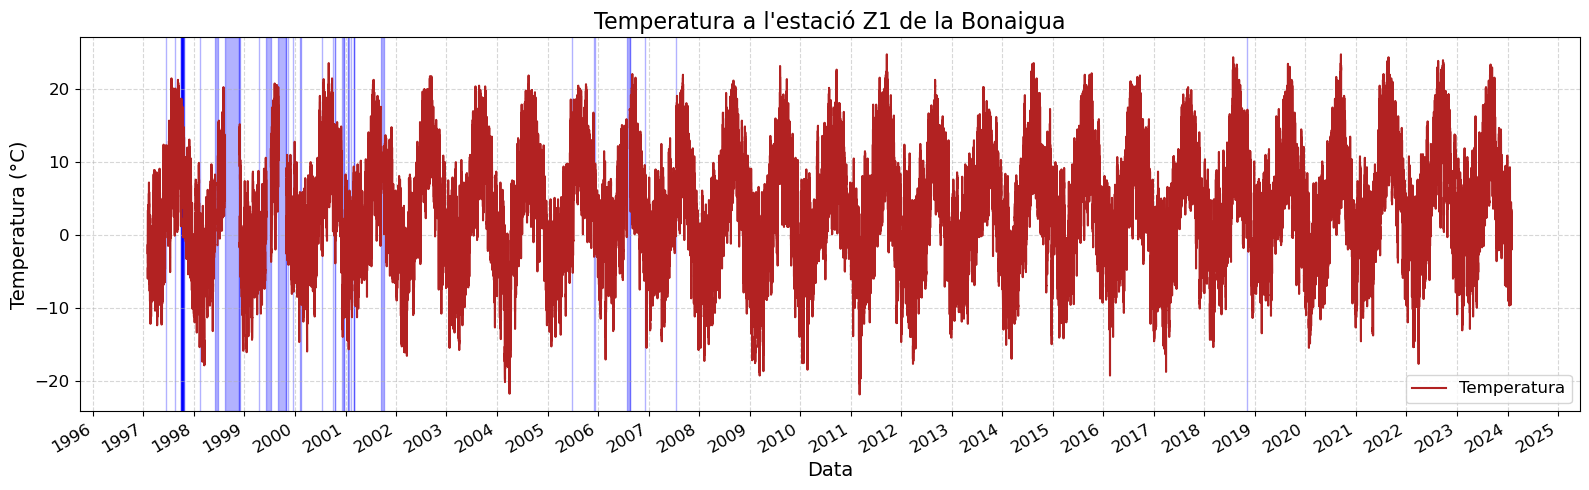
\includegraphics[width=0.75\linewidth]{figures/data_preproces/data_continuitat.png}
    \caption{Sèrie de temperatura horària a l'Estació de la Bonaigua (1998–2024), amb buits de dades destacats.}

    \label{fig:Serie_com_disc}
\end{figure}

% ------------------------------------------------------------
% Fi del document
% ------------------------------------------------------------
\end{document}
